\chapter{Basics}

%%%%%%%%%%%%%%%%%%%%%%%%%%%%%%%%%%%%%%%%%%%%%%%%%%%%%%%%%%%%%%%%%%%%%%%%%%%%%%%
\section{Choice of $\log$ / Determination $\tilde\theta$ of $\theta$}
\textbf{Universal cover:}
\[
  \R\to S^1; \nu \mapsto e^{i\nu}
\]
\begin{center}
  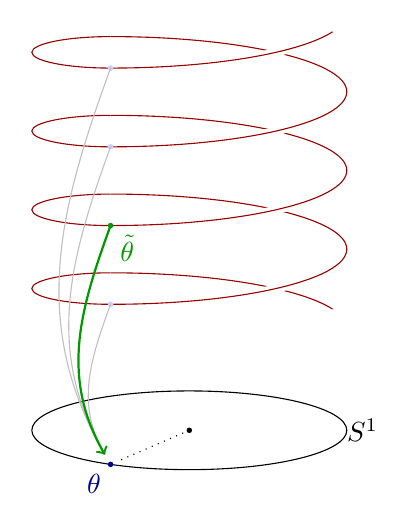
\begin{tikzpicture}[scale=1]
    \node[] (zero) at (0,0) {};
    \fill (zero) circle (1pt);
    \draw (0,-0.5) arc (270:-90:2 and 0.5);

    \node (theta) at ({cos(240) * 2},{sin(240) * 0.5}) {};
    % \node [below left of=theta,blue!40!white] {$\theta$};

    \draw[dotted] (0,0) -- (theta);
    \fill[blue!60!black] (theta) circle (1pt);


    \draw[red!60!black] (-1,2) arc (270:200:-3 and -0.7);
    \draw[line width=3pt,white] (-1,2) arc (270:90:1 and -0.2) arc (270:90:-3 and 0.7);
    \draw[red!60!black] (-1,2) arc (270:90:1 and -0.2) arc (270:90:-3 and 0.7);
    \fill[blue!20!white] (-1,1.6) circle (1pt);

    \draw[line width=3pt,white] (-1,3) arc (270:90:1 and -0.2) arc (270:90:-3 and 0.7);
    \draw[red!60!black] (-1,3) arc (270:90:1 and -0.2) arc (270:90:-3 and 0.7);
    \fill[green!60!black] (-1,2.6) circle (1pt);

    \draw[line width=3pt,white] (-1,4) arc (270:90:1 and -0.2) arc (270:90:-3 and 0.7);
    \draw[red!60!black] (-1,4) arc (270:90:1 and -0.2) arc (270:90:-3 and 0.7);
    \fill[blue!20!white] (-1,3.6) circle (1pt);

    \draw[line width=3pt,white] (-1,5) arc (270:90:1 and -0.2) arc (270:200:-3 and 0.7);
    \draw[red!60!black] (-1,5) arc (270:90:1 and -0.2) arc (270:200:-3 and 0.7);
    \fill[blue!20!white] (-1,4.6) circle (1pt);


    \draw[->,gray!50!white] (-1,1.6) to[out=250,in=120] (theta);
    \draw[->,gray!50!white] (-1,3.6) to[out=250,in=120] (theta);
    \draw[->,gray!50!white] (-1,4.6) to[out=250,in=120] (theta);
    \draw[->,green!60!black,thick] (-1,2.6) to[out=250,in=120] (theta);
    \node[below left,blue!60!black] at (theta) {$\theta$};
    \node[below right,green!60!black] at (-1,2.6) {$\tilde\theta$};

    \node[red!60!black] at (2.2,4.8) {$\R$};
    \node at (2.2,0) {$S^1$};
  \end{tikzpicture}
\end{center}

\textbf{$q$-sheet cover:}

\textbf{multivalued functions:}
\textbf{determination of a function:}
\TODO[principal determination of $x^{1/2}$]

%%%%%%%%%%%%%%%%%%%%%%%%%%%%%%%%%%%%%%%%%%%%%%%%%%%%%%%%%%%%%%%%%%%%%%%%%%%%%%%
\section{Asymptotic analysis}
\begin{comment}
  \begin{multicols}{2}
    ´classical'
    \begin{itemize}
      \item \cite[60]{sabbah_cimpa90} Chapter II.2.2
        \begin{itemize}
          \item \cite{sabbah2000equations}
        \end{itemize}
      \item \textbf{\textcolor{blue}{Van der Put:
            \cite[Chapter 7]{van2003galois}: Exact Asymptotics}}
      \item \cite{majima1984asymptotic}
      \item \cite{Balser2000Formal}
      \item \cite{Loday1994}
      \item \textbf{\textcolor{blue}{\cite{Loday2014} Chapter 2}}
    \end{itemize}
    \columnbreak
    ´sheafical'
    \begin{itemize}
      \item \textbf{\textcolor{red}{\cite[II.5]{sabbah2007isomonodromic}}}
    \end{itemize}
  \end{multicols}
  \TODO[\cite{sibuya1990Linear} Appendix A.3]
\end{comment}
In this chapter, we want to look at asymptotic expansions at $t_0$.
There are various references for Poincarè asymptotic expansions, or for short,
asymptotic expansions.
We will mostly refer to \cite[chapter 2]{Loday2014} and
\cite[chapter 7]{van2003galois}.
\TODO[For the second definition we will also use
\cite{sabbah2007isomonodromic}.]
We will assume, that $t_0=0$ and this is without loss of generality, since
asymptotic expansions at $t_0\in\C$ reduce to asymptotic expansions at $0$
after the change of variable $t\mapsto s=t-t_0$ and asymptotic expansions at
$x_0=\infty$ are obtained via $t\mapsto s=\frac{1}{t}$.

\TODO[Define Sect command]

We introduce the following notations:
\begin{notations} We denote by
  \begin{itemize}
    \item $\mathfrak{s}=\mathfrak{s}_{a,b}(r)$, $a,b\in\S^1$ and $r\in\R_{>0}$
      the open sector
      \[
        \mathfrak{s}_{a,b}(r):=\left\{t\in\C \mid a<\arg(t)<b, 0<|t|<r\right\}
      \]
      of all points $t\in\C$ satisfying $a<\arg(t)<b$ and $0<|t|<r$;
    \item $\mathfrak{s}_{I}(r)=\mathfrak{s}_{a,b}(r)$ for
      $I=(a,b)$\footnote{i.e.\ an open interval of $S^1$} an open arc;
    \item $\bar{\mathfrak{s}}=\bar{\mathfrak{s}}_{a,b}(r)$ the closure of
      $\mathfrak{s}_{a,b}(r)$ in $\C^*:=\C\backslash\{0\}$.
  \end{itemize}
  \begin{center}
    \begin{tikzpicture}[scale=4]
      \node (zero) at (0,0) {};
      \node[below left] at (zero) {$0$};
      \draw[blue,dashed] (zero) circle (1cm);
      \node[blue,right] at (-1,-.7) {$S^1$};

      \filldraw[fill=green!20!white
        ,draw=green!60!black
        ,thick
        ,path fading=west] (0,0)
      -- ({cos( -30 )*.65},{sin( -30 )*.65}) arc (-30:70:.65) -- cycle;
      \draw[blue!60!black,thick] (0,0) -- ({cos( -30 )*.65},{sin( -30)*.65});
      \node[green!40!black] at (.4,.3)
        {$\mathfrak{s}_{\textcolor{red!60!black}{a,b}}
        (\textcolor{blue!60!black}{r})$};
      \node[green!40!black] at (.3,-.25) {$\textcolor{blue!60!black}{r}$};

      \draw[thick,red!60!black] ({cos( -30 )},{sin( -30 )}) arc (-30:70:1);

      \fill[red!60!black] ({cos( -30 )},{sin( -30 )}) circle(.7pt);
      \fill[red!60!black] ({cos( 70 )},{sin( 70 )}) circle(.7pt);

      \node[red!60!black] at ({1.1 * cos(70)},{1.1 * sin(70)}) {$a$};
      \node[red!60!black] at ({1.1 * cos(-30)},{1.1 * sin(-30)}) {$b$};

      \node[red!60!black,right] at (.8,.6) {$I$};

      \fill[white] (zero) circle (1.5pt);
      \fill (zero) circle (.7pt);
    \end{tikzpicture}
  \end{center}
  \TODO[Sectors on the Riemann surface of the logarithm]
\end{notations}
\begin{rem}
  \begin{itemize}
    \item We will say, that \emph{a sector $\mathfrak{s}_{I}(r)$ contains
      $\theta\in S^1$} if $\theta\in I$. In the same way we will say, that
      $\mathfrak{s}_I(r)$ contains $U\subset S^1$ if $U\subset I$ or that
      $U\subset S^1$ contains a sector $\mathfrak{s}_I(r)$ if $I\subset U$.
    \item Since the explicit value $r$ of the radius does not matter, we shall
      simply speak of an \emph{arc} or \emph{interval}
      $U(\theta,\epsilon):=\left(\theta-\frac{\epsilon}{2}
      ,\theta+\frac{\epsilon}{2}\right)\subset S^1$ in place of a sector
      $\mathfrak{s}_{\theta-\frac{\pi}{2k},\theta+\frac{\pi}{2k}}(r)$ for a
      sufficiently small $r$. \TODO[Define via limit]
  \end{itemize}
\end{rem}
\begin{defn}
  A sector $\mathfrak{s}_{a',b'}(r')$ is said to be a proper sub-sector of the
  sector $\mathfrak{s}_{a,b}(r)$,
  $\mathfrak{s}_{a',b'}(r')\Subset\mathfrak{s}_{a,b}(r)$, if its closure
  $\bar{\mathfrak{s}}_{a',b'}(r')$ is included in $\mathfrak{s}_{a,b}(r)$.
  \begin{rem}
    $\mathfrak{s}_{a',b'}(r')\Subset\mathfrak{s}_{a,b}(r)$ if and only if
    \begin{itemize}
      \item[] $a<a'<b'<b$ and $r'<r$.
    \end{itemize}
  \end{rem}
\end{defn}

\begin{defn}
  \def\myN{\textbf{\textcolor{blue!40!black}{N}}}
  \def\mySect{\textcolor{red!40!black}{\mathfrak{s}'}}
  \def\myConst{\textcolor{green!40!black}{C(\myN,\mySect)}}
  A function $f\in\cO(\mathfrak{s})$ is said to \emph{have the formal Laurent
  series $\sum_{n\geq n_0}a_nt^n$ as asymptotic expansion} (or \emph{to be
  asymptotic to the series}) on the sector $\mathfrak{s}$ if
  \begin{itemize}
    \item for all proper sub-sectors $\mySect\Subset\mathfrak{s}$ and
    \item all $\myN\in\N$,
  \end{itemize}
  there exists a constant
  $\myConst$ such that the following estimate\footnote{Sometimes, for example
    in \cite{sabbah_cimpa90}, this condition is written as
    \[
      \lim_{z\to0,z\in{\mySect}}
      |t|^{-(\myN-1)}
      \left|
        f(x)-\sum_{n_0\leq n\leq \myN-1}c_nt^n
      \right|=0
      \qquad \text{ for all } t\in \mySect \,.
    \]} holds
  \[
    \left|
      f(x)-\sum_{n_0\leq n\leq \myN-1}c_nt^n
    \right|
    \leq \myConst|t|^{\myN} \qquad \text{ for all }t\in \mySect \,.
  \]
  \begin{enumerate}
    \item We will say, that \emph{$f$ has the formal Laurent series $\hat g$ as
      asymptotic expansion on the interval $I\subset S^1$} if there exists a
      $r\in\R_{>0}$ such that $f$ has the formal Laurent series $\hat g$ as
      asymptotic expansion on $\mathfrak{s}_I(r)$.
    \item We will say, that \emph{$f$ has the formal Laurent series $\hat g$ as
      asymptotic expansion in the direction $\theta$} if there exists an
      interval $\theta\in I\subset S^1$ such that $f$ has formal Laurent series
      $\hat g$ as asymptotic expansion on the interval $I$.
  \end{enumerate}
\end{defn}
If $f$ has $\hat g$ as asymptotic expansion on the sector $\mathfrak{s}$ (or on
the interval $I\subset S^1$, or in the direction $\theta$), we denote that by
$f\sim_{\mathfrak{s}}\hat g$ (or $f\sim_{I}\hat g$, or $f\sim_{\theta}\hat g$).
\begin{defn}
  \begin{enumerate}
    \item Define $\cA(\mathfrak{s})$ as the set of holomorphic functions
      $f\in\cO(\mathfrak{s})$ which admit an asymptotic expansion at $0$ on
      $\mathfrak{s}$.
      \begin{rem}
        \begin{enumerate}
          \item $\cA(\mathfrak{s})$ is a subring of $\cO(\mathfrak{s})$.
          \item $\cA(\mathfrak{s})$ contains $\C(\!\{t\}\!)$ as a subfield.
        \end{enumerate}
      \end{rem}
    \item Define $\cA(a,b)\!\!\overset{(a,b)=I}{=}\!\!\cA(I)$
      as the limit $\underset{r\to0}{\underrightarrow{\lim}}
      \cA(\mathfrak{s}_{a,b}(r))$\footnote{In more detail this means that the
        elements of $\cA(a,b)$ are pairs $(f,\mathfrak{s}_{a,b}(r))$ mit
        $f\in\cA(\mathfrak{s}_{a,b}(r))$. The equivalence relation is given by
        $(f_1,\mathfrak{s}_{a,b}(r_1))\sim(f_2,\mathfrak{s}_{a,b}(r_2))$ if
      there is a pair $(f_3,\mathfrak{s}_{a,b}(r_3))$ such that
      $r_3<\min(r_1,r_2)$ and $f_3=f_1=f_2$ on $\mathfrak{s}_{a,b}(r_3)$.}.
  \end{enumerate}
\end{defn}
It can easily be seen, that $\cA:U\to\cA(U)$ defines a sheaf on $S^1$.

\TODO[Properties,Examples,\dots]
\begin{defn}
  \begin{itemize}
    \item One writes
      \[
        T_{I}:\cA(I)\to\C(\!(t)\!)
        \qquad\left(\text{resp.}\qquad
        T_{\mathfrak{s}}:\cA(\mathfrak{s})\to\C(\!(t)\!)\qquad\right)
      \]
      for the mapping, called \emph{Taylor map}, which associates to each
      function $f\in\cA(I)$ (resp.\ $f\in\cA(\mathfrak{s})$) its asymptotic
      expansion.
    \item A function $f$ with $T_{\mathfrak{s}}(f)=\id_{\mathfrak{s}}$ is
      called \emph{flat (on $\mathfrak{s}$)}. \TODO[resp]
    \item Denote by $\cA^{<0}(I)$ (resp.\ $\cA^{<0}(\mathfrak{s})$) the set
      $\ker(T_{I})\subset\cA(I)$ (resp.\
      $\ker(T_{\mathfrak{s}})\subset\cA(\mathfrak{s})$) of functions asymptotic
      to zero at $0$.
  \end{itemize}
\end{defn}
The kernel $\cA^{<0}(I)$ is not zero.
Let $I=\left(-\frac{\pi}{2},\frac{\pi}{2}\right)$, then $\cA^{<0}(I)$ has the
element $e^{-\frac{1}{\sqrt{t}}}$ where $\sqrt{t}$ stands for the principal
determination of $x^{\frac{1}{2}}$.

\begin{exmp}[Trivial example]
  \marginnote{\cite[Exmp.2.2.3]{Loday2014}}
  If $f$ is an analytic function on $D=\{t\mid |t|<r\}$ then $f$ is asymptotic
  to its Taylor series at $0$ on $D^*=D\backslash\{0\}$. Reciprocally, if $f$
  is an analysis on $D^*$ that has an asymptotic expansion at $0$ on $D^*$
  then, $f$ is bounded near $0$ and according to the removable singularity
  theorem, $f$ is analytic on $D$.
  \begin{rem}
    This implies, that $\cA(S^1)\cong\C(\!\{t\}\!)$.
  \end{rem}
\end{exmp}
For more examples see Loday-Richauds book \cite{Loday2014}
\cite[Exmp.2.2.4]{Loday2014}, \cite[Exmp.2.2.5]{Loday2014},
\cite[Exmp.2.2.6]{Loday2014}, \cite[Exmp.2.2.7]{Loday2014} and
\cite[Exmp.2.2.8]{Loday2014}.
\begin{comment}
  \begin{exmp}[Fundamental example: the Euler function]
    \marginnote{\cite[Exmp.2.2.4]{Loday2014}}
    Consider the Euler equation
    \begin{equation}
      x^2\frac{dy}{dx}+y=x \,.
    \end{equation}
    \TODO[]
  \end{exmp}
  \begin{exmp}[Classical example: the exponential integral]
    \marginnote{\cite[Exmp.2.2.5]{Loday2014}}
    Consider the exponential integral
    \begin{equation}
      Ei(x)=\int_x^{+\infty}e^{-t}\frac{dt}{t} \,.
    \end{equation}
    \TODO[]
  \end{exmp}
  \begin{exmp}[A generalized hypergeometric series ${}_3F_0$]
    \marginnote{\cite[Exmp.2.2.6]{Loday2014}}
    \TODO[]
  \end{exmp}
  \begin{exmp}[A series of a mild difference equation]
    \marginnote{\cite[Exmp.2.2.7]{Loday2014}}
    \TODO[]
  \end{exmp}
  \begin{exmp}[A series of a wild difference equation]
    \marginnote{\cite[Exmp.2.2.8]{Loday2014}}
    \TODO[]
  \end{exmp}
\end{comment}

\begin{rem}
  Let $I\subset S^1$ be a arc.
  Let $f$, $f_1$ and $f_2$ be functions which satisfy $f\sim_I\hat f$,
  $f_1\sim_I\hat f_1$ and $f_2\sim_I\hat f_2$.
  We have the rules:
  \begin{enumerate}
    \item \cite[4.5.Thm.13]{Balser2000Formal}:
      $f_1(t)+f_2(t)$ is on $I$ asymptotic to $\hat f_1(t)+\hat f_2(t)$.
    \item \cite[4.5.Thm.14]{Balser2000Formal}:
      $f_1(t)f_2(t)$ is on $I$ asymptotic to $\hat f_1(t)\hat f_2(t)$.
    \item \cite[4.5.Thm.20]{Balser2000Formal}:
      \begin{enumerate}
        \item $f'(t)$ is on $I$ asymptotic to $\hat f'(t)$.
        \item $\int_0^tf(s)\,ds$ is on $I$ asymptotic to $\int_0^t\hat f(t)\,ds$.
      \end{enumerate}
    \item \cite[4.5.Thm.21]{Balser2000Formal}:
      \marginnote{\cite[II.2.2.4]{sabbah_cimpa90}}
      if $f\in\cA(I)\backslash\cA^{<0}(I)$ then
      $f^{-1}(t)$ is on $I$ asymptotic to $\hat f^{-1}(t)$.
  \end{enumerate}
  \TODO[Better source/proofs?]
\end{rem}
\begin{lem}
  $\cA(I)$ is stable under derivation.
\end{lem}
\begin{proof}
  Let $f\in\cA(I)$ with asymptotic expansion $\hat f=\sum_{-n_0\leq n}a_nx^n$
  its asymptotic expansion where we assume that $n_0=0$.
  One has for each $m\geq0$
  \[
    f(t)=\sum_{n=0}^ma_nt^n+R_m(t)t^m
  \]
  with $\underset{\substack{t\to0\\t\in\mathfrak{s}_I(r)}}{\lim}R_m(t)=0$.
  This implies that $R_m$ is holomorphic in $\mathfrak{s}_I(r)$.
  Thus one has
  \[
    f'(t)=\sum_{n=0}^mna_nt^{n-1}+mR_m(t)t^{m-1}+R_m'(t)t^m
  \]
  Let $C_{x,\rho}$ be the circle at $x$ with radius $\rho$ contained in
  $\mathfrak{s}_I(r)$. The Cauchy theorem implies then, that
  \[
    |R_m'(t)|\leq\frac{1}{\rho}\max_{s\in\C_{x,\rho}}|R(s)| \,.
  \]
  Let $J$ be a relativly compact open set in $I$, then there exists a positive
  number $\alpha$ such that for all $x\in\mathfrak{s}_I(r)$ one has
  $C_{x,\alpha|x|}\subset\mathfrak{s}_I(r)$.
  \TODO{}
  This proves that $\hat{f'}$ is an asymptotic expansion for $f'$ in
  $\mathfrak{s}_I(r)$.
\end{proof}

\subsection{Borel-Ritt Lemma}
\begin{comment}
  \begin{itemize}
    \item \cite[Lem.II.2.2.5]{sabbah_cimpa90}: $T_I$
    \item \textbf{\cite[Th.7.3]{van2003galois}}: $T_I=T_{(a,b)}$
    \item \cite[Th.2.4.1]{Loday2014}: $T_{\mathfrak{s}}$
    \item \cite[4.4.Thm.16]{Balser2000Formal}
  \end{itemize}
\end{comment}
The most important theorem here is the Borel-Ritt lemma.
\begin{thm}[Borel-Ritt]
  \label{thm:borel-ritt}
  Let $I$ be an open arc with a opening less than $2\pi$. Then the Taylor map
  \[
    T_{I}:\cA(I)\to\C(\!(t)\!)
  \]
  is onto.
\end{thm}
There are multiple approaches to obtain a function $f\in\cA(I)$ asymptotic to a
given function $\hat f\in\C(\!(t)\!)$ in a canonical way. For example
(multi-)multisummability which is detailed described in~\cite{Loday2014}.
\begin{proof}[Proof of thm~\ref{thm:borel-ritt}]
  Let $I:=(-\pi,\pi)$ and $R\in\R_{>0}$.
  We will prove this for the sector
  \[
    \mathfrak{s}:=\mathfrak{s}_{I}(R)=\left\{
      t\in\C\mid |\arg(t)|<\pi, 0<|t|<R
    \right\}
  \]
  in which, after rotation and for large enough $R$, every sector
  $\mathfrak{s}''\subsetneq\C^*$ lies.
  Let $\sum a_nz^n$ be a formal Laurent series. We look for a function
  $f\in\cA(I)$ with Taylor series $T_{I}f=\sum a_nz^n$.
  By subtracting the principal part\TODO[?] we may assume, that this series has
  no terms with negative degree.
  Let $b_n$ be a sequence, which satisfies
  \begin{itemize}
    \item[] the series $\sum |a_n|b_nR^{n-\frac{1}{2}}$ is convergent.
  \end{itemize}
  For example\TODO[realy?], one may set
  \[
    b_n=\begin{cases}
      0                 & \text{when~} n=0
      \\\frac{1}{n!}|a_n| & \text{when~} n>0
    \end{cases}
  \]
  Let $\sqrt{t}$ be the branch of the square root function, that satisfies
  $|\arg(\sqrt{t})|<\frac{\pi}{2}$\footnote{For $t=re^{i\phi}$ is
  $\sqrt{t}=\sqrt{r}e^{i\frac{\phi}{2}}$ with $-\pi<\phi<\pi$.} for all
  $t\in\mathfrak{s}$.
  For any real number $b_n$, the function
  $\beta_n(t):=1-e^{-\frac{b_n}{\sqrt{t}}}$ satisfies
  \begin{enumerate}
    \item[(a)] $|\beta_n(t)|\leq\frac{b_n}{\sqrt{|t|}}$ since
      $1-e^t=-\int_0^te^s\,ds$ implies that $|1-e^t|<|t|$ for $\Re(t)<0$ and
    \item[(b)] $\beta_n$ has asymptotic expansion $1$ on $\mathfrak{s}$ (thus
      $\beta_n-1$ has asymptotic expansion $0$ on $\mathfrak{s}$).
  \end{enumerate}
  Define $f(t)=\sum a_n\beta_n(t)t^n$.
  Since 
  \[
    |a_n\beta_n(t)t^n|
    \leq|a_n|b_n|z|^{n-\frac{1}{2}}
    \leq|a_n|b_nR^{n-\frac{1}{2}},
  \]
  the series
  $\sum a_n\beta_n(t)t^n$ converges and its sum $f(t)$ is in
  $\cO(\mathfrak{s})$.

  Consider a propper sub-sector $\mathfrak{s}'\Subset\mathfrak{s}$ and
  $t\in\mathfrak{s}'$. Then, for every $N>0$
  \begin{align*}
    \left|f(t)-\sum_{n=0}^{N-1} a_nt^n\right| 
    &\leq \left| \sum_{n=0}^{N-1}a_n(\beta_n(t)-1)t^n \right|
      +|t|^N\sum_{n\geq N}\left| a_n\beta_n(t)t^{n-N} \right|
  \\&= \left| \sum_{n=0}^{N-1}a_ne^{-\frac{b_n}{\sqrt{t}}}t^n \right|
      +|t|^N\sum_{n\geq N}\left| a_n\beta_n(t)t^{n-N} \right|
  \end{align*}
  The first summand is a finite sum of terms, which are all asymptotic to $0$
  and then, is majorized by $C'|t|^N$ for a convenient constant $C'$.
  The second summand is majorized by
  \[
    |t|^N\left(2|a_n|+\sum_{n\geq N+1}|a_n|b_nR^{n-\frac{1}{2}-N}\right).
  \]
  By setting $C=C'+2|a_n|+\sum_{n\geq N+1}|a_n|b_nR^{n-\frac{1}{2}-N}$ we
  obtain a positive constant $C$, which depends on $N$ and the radius of
  $\mathfrak{s}'<R$, such that 
  \[
    \left|f(t)-\sum_{n=0}^{N-1} a_nt^n\right| \leq C|t|^N
    \qquad\text{ for all } t\in\mathfrak{s}' \,.
  \]

  \TODO[The GENERAL CASE: see \cite{Loday2014} page 28]
\end{proof}

\begin{comment}
%%%%%%%%%%%%%%%%%%%%%%%%%%%%%%%%%%%%%%%%%%%%%%%%%%%%%%%%%%%%%%%%%%%%%%%%%%%%%%%
  \subsection{Sheaf definition from \cite{sabbah2007isomonodromic}}
  See \cite[II.5.c]{sabbah2007isomonodromic}.
  Let
  \begin{itemize}
    \item $D$ the open disc with coordinate $t$ centered at the origin and of
      radius $r^0>0$.
    \item $\tilde D:=[0,r^0[\times S^1$
    \item $\pi:\tilde D\to D,~(r,\theta)\mapsto t=re^{i\theta}$ 
  \end{itemize}
  \dots we can define the derivations $t\partial/\partial t$ and 
  $\bar t\partial/\partial\bar t$.
  \begin{defn}
    The sheaf of rings $\cA_{\tilde D}$ is defined as the subsheaf of
    $\sC_{\tilde D}^\infty$ of germs killed by $\bar t\partial/\partial\bar t$.
  \end{defn}
  \begin{rem}
    \cite{sabbah2007isomonodromic}: Remark 5.11
  \end{rem}
  \begin{rem}
    On the sheaf $\cA_{\tilde D}$ is defined the action of the derivation
    $\partial/\partial t$\dots
  \end{rem}
  \dots
\end{comment}
